\documentclass[letterpaper, 12pt]{article}

\setlength{\topmargin}{0in}
\setlength{\headheight}{0in}
\setlength{\headsep}{0in}
\setlength{\footskip}{0.5in}
\setlength{\textheight}{\paperheight}
\addtolength{\textheight}{-2in}
\addtolength{\textheight}{-\footskip}

\setlength{\oddsidemargin}{0in}
\setlength{\evensidemargin}{0in}
\setlength{\textwidth}{\paperwidth}
\addtolength{\textwidth}{-2in}

\pagestyle{empty}

\usepackage{amsfonts}
\usepackage{tikz}

\begin{document}

\begin{center}
\bfseries
San Jos\'{e} State University \\
Fall 2015 \\
Math-8: College Algebra \\
Section 03: MW noon--1:15pm \\
Section 05: MW 4:30--5:45pm \\
\bigskip
Quiz \#14 (Solutions)
\end{center}

\bigskip

1. We saw in class that $a^x$ for $x\in\mathbb{R}$ is the value that $a^x$
approaches as we get closer and closer to $x$ with a sequence of rational
numbers. This works for the base as well. We were also introduced to the
special base $e=2.71828\ldots$, known as Euler's number. Calculate $e^2$ on
your calculator and show how $2^2$, $2.7^2$, $2.71^2$, \ldots approaches
$e^2$. Look at 6 such terms.

\bigskip

\begin{eqnarray*}
e &=& 2.71828 \\
e^2 &=& 7.38906 \\
\end{eqnarray*}

\begin{tabular}{|c|c|}
\hline
2 & 4 \\
\hline
2.7 & 7.29 \\
\hline
2.71 & 7.3441 \\
\hline
2.718 & 7.38752 \\
\hline
2.7182 & 7.38861 \\
\hline
2.71828 & 7.38905 \\
\hline
\end{tabular}

\bigskip

2. Sketch the graph: $y=e^{-x+2}+1$. (Hint: factor out the negative in the
exponent first).

\[y=e^{-(x-2)}+1\]

\bigskip

Start with the basic graph $y=e^x$.

\bigskip

\begin{center}
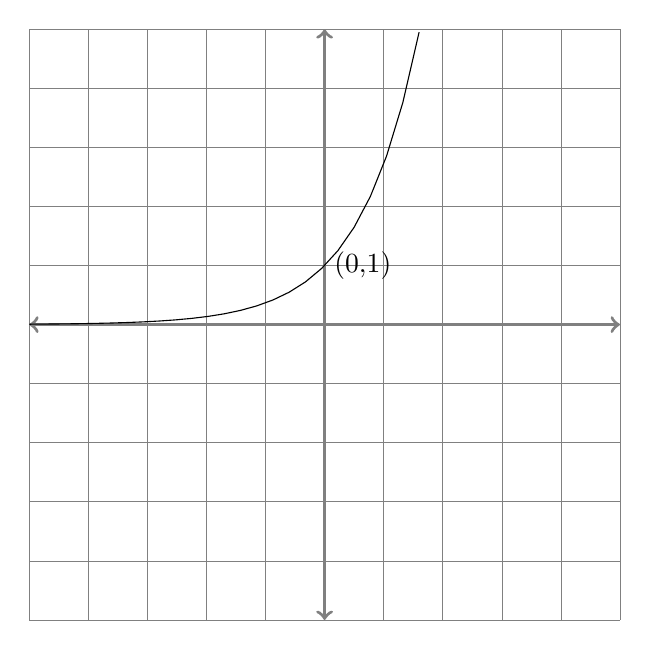
\begin{tikzpicture}[scale=0.75]
\draw [help lines] (-5,-5) grid (5,5);
\draw [help lines, <->, very thick] (-5,0) -- (5,0);
\draw [help lines, <->, very thick] (0,-5) -- (0,5);
\node [right] at (0,1) {(0,1)};
\draw [domain=-5:1.6] plot (\x, {e^(\x)});
\end{tikzpicture}
\end{center}

\bigskip

Translate right by 2.

\bigskip

\begin{center}
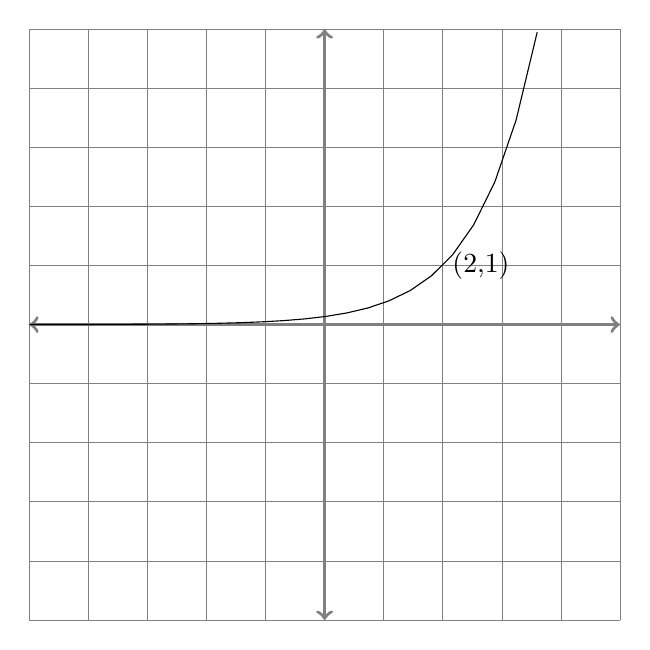
\begin{tikzpicture}[scale=0.75]
\draw [help lines] (-5,-5) grid (5,5);
\draw [help lines, <->, very thick] (-5,0) -- (5,0);
\draw [help lines, <->, very thick] (0,-5) -- (0,5);
\node [right] at (2,1) {(2,1)};
\draw [domain=-5:3.6] plot (\x, {e^((\x)-2)});
\end{tikzpicture}
\end{center}

\bigskip

Reflect across the x-axis.

\bigskip

\begin{center}
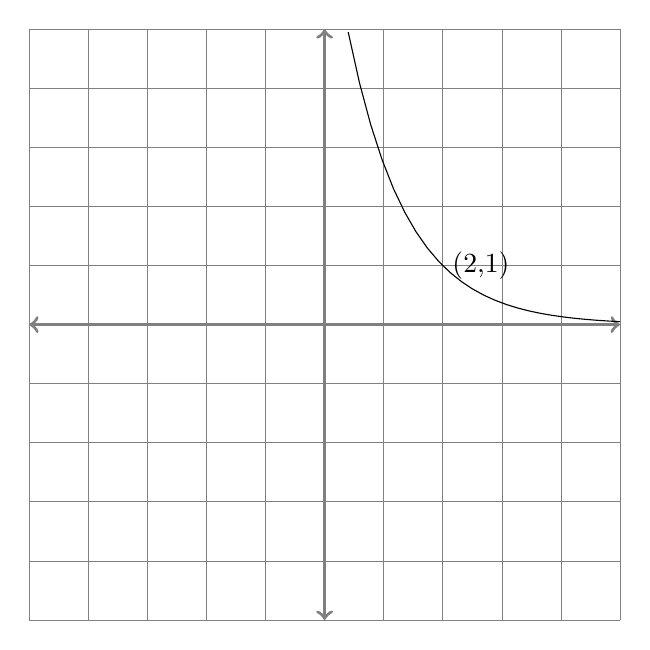
\begin{tikzpicture}[scale=0.75]
\draw [help lines] (-5,-5) grid (5,5);
\draw [help lines, <->, very thick] (-5,0) -- (5,0);
\draw [help lines, <->, very thick] (0,-5) -- (0,5);
\node [right] at (2,1) {(2,1)};
\draw [domain=0.4:5] plot (\x, {e^-((\x)-2)});
\end{tikzpicture}
\end{center}

\bigskip

Finally, translate up by 1.

\bigskip

\begin{center}
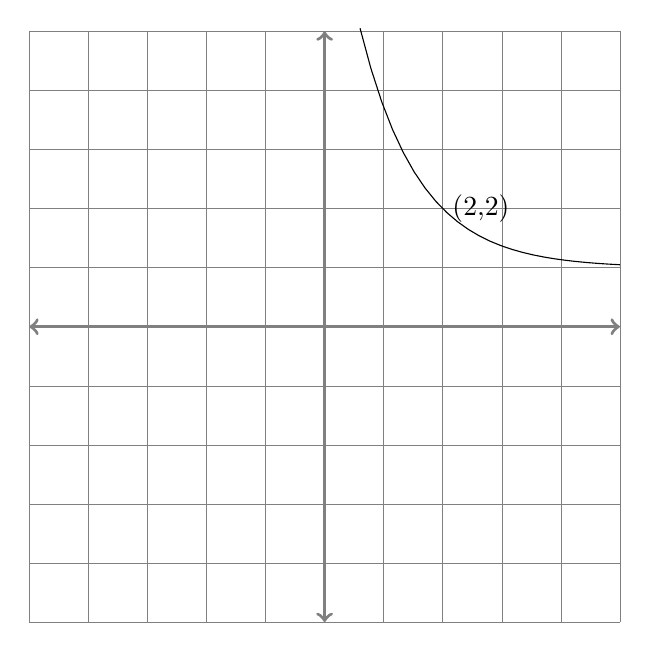
\begin{tikzpicture}[scale=0.75]
\draw [help lines] (-5,-5) grid (5,5);
\draw [help lines, <->, very thick] (-5,0) -- (5,0);
\draw [help lines, <->, very thick] (0,-5) -- (0,5);
\node [right] at (2,2) {(2,2)};
\draw [domain=0.6:5] plot (\x, {e^-((\x)-2)+1});
\end{tikzpicture}
\end{center}

\bigskip

3. Determine the amount of money in a savings account after 5 years at a yearly
interest rate of 2\% assuming that the original principle is \$10000 and the
compounding rate is: a) monthly, and b) continuous.

\bigskip

a. n=12

\[A = 10000\left(1+\frac{0.02}{12}\right)^{5\cdot12} = \$11050.80\]

b. Continuous

\[A = 10000e^{0.02\cdot5} = \$11051.70\]

\bigskip

4. The half-life of Uranium-235 is about 700 million years. What percent of a
sample is left after only 100 million years?

\bigskip

\[\frac{A}{A_0}=\left(\frac{1}{2}\right)^{\frac{100}{700}}=0.906=90.6\%\]

\bigskip

5. Evaluate:

\bigskip

a. $\log_2 256=8$

\bigskip

b. $\log_{10} 10000=4$

\bigskip

c. $\ln 5=1.6094$

\bigskip

6. Solve:

\bigskip

a. $\log_3(x+1)=\log_3(13)$.

\begin{eqnarray*}
\log_3(x+1) &=& \log_3(13) \\
x+1 &=& 13 \\
x &=& 12 \\
\end{eqnarray*}

Before we state the final answer we need to plug it back in to the original
equation and make sure that no domains are violated, and indeed, everything is
OK here.  So, $x=12$.

\bigskip

b. $10\log_7(7^{x-2})=5^{\log_5(2x-1)}$

\begin{eqnarray*}
10\log_7(7^{x-2}) &=& 5^{\log_5(2x-1)} \\
10(x-2) &=& 2x-1 \\
10x-20 &=& 2x-1 \\
8x &=& 19 \\
x &=& \frac{19}{8} \\
\end{eqnarray*}

Thus, there is no solution.

\bigskip

7. Determine the domain for $f(x)=\frac{\log_3(x^2+7x+12)}{\sqrt{x-1}}$

\bigskip

There are two domain issues that need to be checked: the $log$ in the numerator
and the square root in the denominator.  For the $log$ in the numerator, we
must eliminate negative and zero values:

\[x^2+7x+12=(x+4)(x+3)>0\]

So we have critical points -4 and -3.  Using a sign table to check the
intervals:

\bigskip

\begin{tabular}{c|cc|c}
& (x+3) & (x+4) & \\
\hline
-5 & $-$ & $-$ & $+$ \\
-3.5 & $-$ & $+$ & $-$ \\
0 & $+$ & $+$ & $+$ \\
\end{tabular}

\bigskip

\begin{center}
\begin{tikzpicture}[scale=1]
\draw (-5,0) -- (-2,0);
\draw (-4,0.1) -- (-4,-0.1);
\draw (-3,0.1) -- (-3,-0.1);
\node [below] at (-4,0) {-4};
\node [below] at (-3,0) {-3};
\node [above] at (-4.5, 0) {+};
\node [above] at (-3.5, 0) {-};
\node [above] at (-2.5, 0) {+};
\end{tikzpicture}
\end{center}

\bigskip

The resulting domain is $(-\infty,-4)\cup(-3,\infty)$.  Note that we do not use
the points -4 and -3, since $log$ does not allow 0.

\bigskip

Now, the denominator requires that $x-1>0$, or $x>1$.  The final domain is the
intersection of these two regions.  Note that the $x>1$ dominates - nothing
equal to or less than -1 is allowed due to the denominator. So the final
answer is $(1, \infty)$.

\bigskip

Note that one of the limitations totally dominating the other is not always the
case.  Sometimes the intersection is more complicated, so don't assume.

\end{document}
